
\documentclass{article}

\usepackage{amsmath}
\usepackage{bm}
\usepackage{graphicx}
\usepackage{helvet}
\usepackage{setspace}

\newcommand{\B}[1]{\textbf{#1}}
\newcommand{\PLOT}[1]{Figure~\ref{plot:#1}}
\newcommand{\TABLE}[1]{Table~\ref{table:#1}}

\begin{document}

\title{Well-Read Gentlemen's Book Scores: 2021-2022}
\author{Justin M. Wozniak and Jamie Antonelli}
\date{December 12, 2022}

\onehalfspacing

\maketitle

\begin{abstract}
\noindent Here we present the results of the 2021-2022 Well-Read Gentlemen's Book Club Survey.
\end{abstract}

\noindent Over the summer of 2022 we conducted a survey\footnote{
{\sffamily https://docs.google.com/forms/d/1cYvzmk2i9iT9OgV8YFXNERlN4\_qC5xMr2Hpz2gqxtig}} to determine the best and most controversial books for the 2021-2022 club year, including the 3-month pilot run in Spring 2021.
We received $N=6$ responses.  The books read are listed in \TABLE{books}.

\begin{table}
  \begin{tabular}{llll}
    \B{Date} & \B{Abbrev.} & \B{Title} & \B{Author} \\ \hline \hline
    \B{2021} & & & \\
    Apr.  6  & \B{Screwtape} & The Screwtape Letters & C.S. Lewis \\
    May   4  & \B{Leibowitz} & A Canticle for Leibowitz & Walter Miller \\
    Jun.  1  & \B{Silence} & Silence & Shusako Endo \\
    Sep.  8  & \B{C\&P} & Crime and Punishment & Fyodor Dostoyevski \\
    Oct. 11  & \B{Ender's} &  Ender's Game & Orson Scott Card \\
    Nov.  8  & \B{Love-Ruins} & Love in the Ruins & Walker Percy \\
    Dec. 13  & \B{Leopard} & The Leopard & Giuseppe di Lampedusa \\
    \B{2022} & & & \\
    Jan. 10  & \B{Faces} & Til We Have Faces & C.S. Lewis \\
    Feb.  7  & \B{Lear} & King Lear & William Shakespeare \\
    Mar. 14  & \B{Iliad} & Iliad & Homer \\
    Apr. 11  & \B{Confessions} & Confessions & St. Augustine \\
    May   9  & \B{Violent} & The Violent Bear it Away & Flannery O'Connor \\
  \end{tabular}
  \caption{Table of books. \label{table:books}}
\end{table}

The main question asked was ``How would you score each of the books we've read with respect to the purposes of the group?''  The question was on a scale of 1-5, with 5 as best.  Averages and standard deviations are shown in \PLOT{scores}.  As shown in the plot, Faces scored the highest.

\newcommand{\plotwidth}{0.9}

\begin{figure}
\includegraphics[width=\plotwidth\columnwidth]{scores}
\caption{Book scores and standard deviations.
  \label{plot:scores}}
\end{figure}

Standard deviations for the same question are shown in \PLOT{stddevs}.  As shown in the plot, Ender's was the most controversial book.

\begin{figure}
\includegraphics[width=\plotwidth\columnwidth]{stddevs}
\caption{Book standard deviations.
  \label{plot:stddevs}}
\end{figure}

The whole data set may be visualized in \PLOT{viz}.  The books are shown in calendar order, and the number of votes at each score level for each book may be seen from left to right.  The averages are marked with a \pmb{\textbar}.  Columns show the number of votes for that score each book received.

\begin{figure}
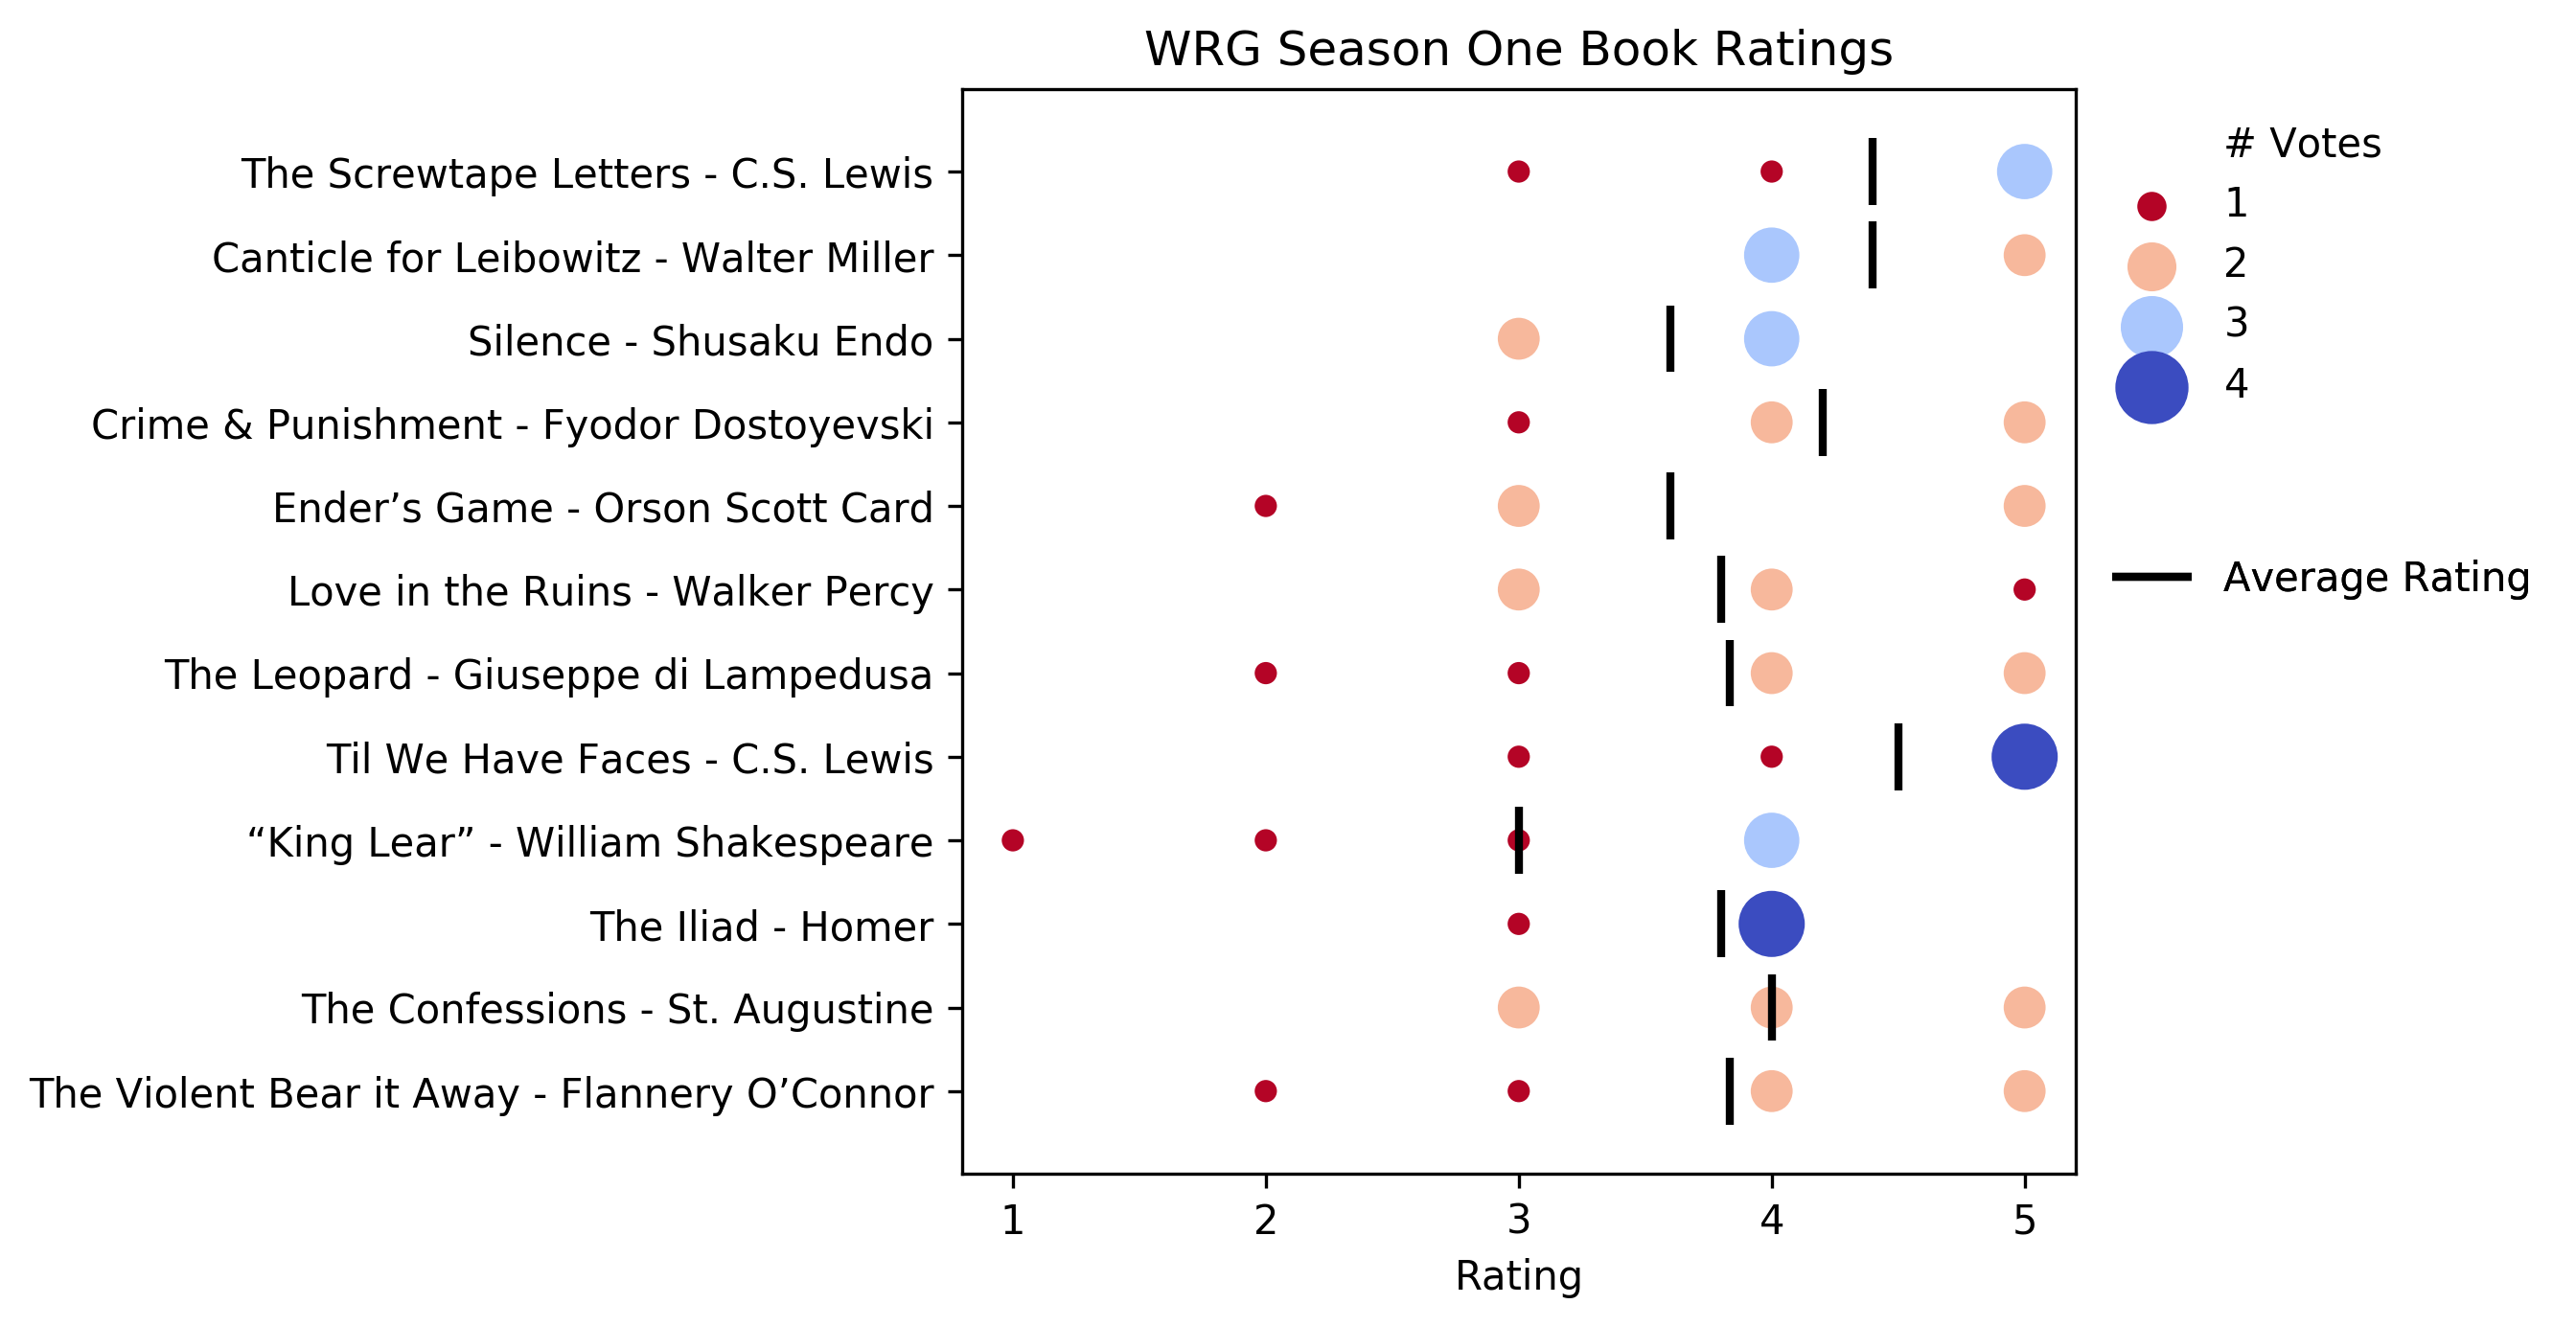
\includegraphics[width=\plotwidth\columnwidth]{viz}
\caption{Book score visualization.
  \label{plot:viz}}
\end{figure}

We also collected numbers on book completion and attendance but due to low $N$ they are not notable.

In the future, we plan to split the question into three: A) a score based on personal preferences, B) a score based on appropriateness, and C) a score based on discussion quality.  We also plan to refine the score from a 5-point scale to a 10-point scale for better resolution.

\end{document}
